%-----------------------------------------------------------------------
% Beginning of chap2.tex
%-----------------------------------------------------------------------
%
%  AMS-LaTeX sample file for a chapter of a monograph, to be used with
%  an AMS monograph document class.  This is a data file input by
%  chapter.tex.
%
%  Use this file as a model for a chapter; DO NOT START BY removing its
%  contents and filling in your own text.
% 
%%%%%%%%%%%%%%%%%%%%%%%%%%%%%%%%%%%%%%%%%%%%%%%%%%%%%%%%%%%%%%%%%%%%%%%%


\chapter*{Lecture 9}
\addcontentsline{toc}{chapter}{Lecture 9}
\addtocounter{chapter}{9}
\addtocounter{section}{0}
%\numberwithin{section}{chapter}
\numberwithin{equation}{chapter}
\numberwithin{theorem}{chapter}

%\epigraph{}{--- \textup{}}

Linear programming duality associates to a linear programming problem a \textbf{dual problem}, with the property that the optimal values of the original and of the dual problem coincide. Duality is an important tool in applications and in the design of algorithms. Linear programming duality rests upon an important family of results in convex geometry, known collectively as Farkas' Lemma.

\section{Farkas' Lemma}

Recall the definition of a convex cone. This is a set $C$ such that for all $\vct{x},\vct{y}\in C$ and $\lambda_1,\lambda_2\geq 0$ we have $\lambda_1\vct{x}+\lambda_2\vct{y}\in C$. 

\begin{lemma}(Hyperplane separation for cones)\label{le:hypcone}
 Let $C\neq \R^n$ be a closed convex cone and $\vct{z}\not\in C$. Then there exists a linear hyperplane such that $C\subseteq H_-$ and $\vct{z}\in \inter H_+$.
\end{lemma}

\begin{figure}[h!]
\centering
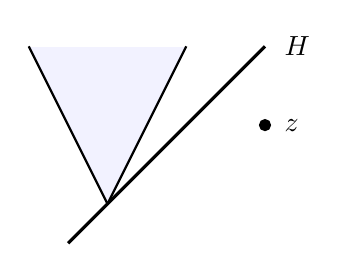
\begin{tikzpicture}[scale=1]
\node (A1) at (2,1)  [label=0:{$\vct{z}$}] {};
\node (A2) at (2,2)  [label=0:{$H$}] {};
\node (A1) at (0,1)  [label=90:{$C$}] {};
\draw[color=black!0, fill=blue!5] (0,0)--(1,2)--(-1,2)--(0,0);
\draw[color=black,thick] (0,0)--(1,2);
\draw[color=black,thick] (0,0)--(-1,2);
\draw[color=black,very thick] (-0.5,-0.5)--(2,2);
\filldraw[black] (2,1) circle (2pt);
\end{tikzpicture}
\caption{Separating hyperplane for a cone} \label{fig:sepcone}
\end{figure}

\begin{proof}
 From Lecture 7 we know that there exists an affine hyperplane $H^{a}$ separating $C$ and $\vct{z}$. Let this affine hyperplane be given by 
 $\ip{\vct{a}}{\vct{x}}=b$.
 We would like to show that $H=\{\vct{x}\mid \ip{\vct{a}}{\vct{x}}=0\}$ is a linear hyperplane separating $C$ and $\vct{z}$.
 From $\ip{\vct{a}}{\vct{z}}>b$ we clearly get $\ip{\vct{a}}{\vct{z}}>0$. Also, $\vct{0}\in H_-$, since $\ip{\vct{a}}{\vct{0}}=0$. Assume now that there exists a point $\vct{x}\in C$ such that $\ip{\vct{a}}{\vct{x}}=c>0$. Since $C$ is a cone, for all $\lambda>0$ we have that $\lambda\vct{x}\in C$. Choosing $\lambda$ so that $\lambda>b/c$ we get 
 \begin{equation*}
  \ip{\vct{a}}{\lambda\vct{x}}=\lambda c>b,
 \end{equation*}
in contradiction to $C\subset H^{a}_-$. This shows that $H$ is a linear separating hyperplane.
\end{proof}


\begin{theorem}(Farkas' Lemma)\label{thm:farkas}
Given a matrix $\mtx{A}\in \R^{m\times n}$ and $\vct{b}\in \R^m$, there
 exists a vector $\vct{x}$ such that
 \begin{equation*}
  \mtx{A}\vct{x}=\vct{b}, \quad \vct{x}\geq 0
 \end{equation*}
if and only if there is not $\vct{y}\in \R^m$ such that
\begin{equation*}
 \mtx{A}^{\trans}\vct{y}\geq \zerovct, \quad \ip{\vct{y}}{\vct{b}}<0. 
\end{equation*}
\end{theorem}

\begin{proof}
Assume $\mtx{A}\vct{x}=\vct{b}$ has a solution $\vct{x}\geq 0$. Then for any $\vct{y}\neq \zerovct$ such that $\mtx{A}^{\trans}\vct{y}\geq \zerovct$,
\begin{equation*}
 0\leq \ip{\mtx{A}^{\trans}\vct{y}}{\vct{x}}=\ip{\vct{y}}{\mtx{A}\vct{x}}=\ip{\vct{y}}{\vct{b}},
\end{equation*}
which shows that $\mtx{A}^{\trans}\vct{y}\geq \zerovct$ and $\ip{\vct{y}}{\vct{b}}<0$ are not simultaneously possible. 

 Assume now that $\mtx{A}\vct{x}=\vct{b}$ has no solution that satisfies $\vct{x}\geq 0$. Let $\vct{a}_1,\dots,\vct{a}_n$ be the columns of $\mtx{A}$. The set of $\mtx{A}\vct{x}$ for $\vct{x}\geq \zerovct$ is the set
 of all nonnegative linear combinations
 \begin{equation*}
  C=\{\vct{z}\in \R^m \mid \vct{z} = x_1\vct{a}_1+\cdots +x_n\vct{a}_n, \ x_i\geq 0\},
 \end{equation*}
and this set is a convex cone. The assumption that there is no nonnegative $\vct{x}$ such that $\mtx{A}\vct{x}=\vct{b}$ means that $\vct{b}\not\in C$. By Lemma~\ref{le:hypcone}, there exists a linear hyperplane $H=\{\vct{x} \mid \ip{\vct{y}}{\vct{x}}=0\}$ such that $C\in H_-$ and $\vct{b}\in \inter H_+$. Formulated differently, there exists a $\vct{y}\in \R^m$ such that
\begin{equation*}
 \forall \vct{z}\in C\colon \ip{\vct{z}}{\vct{y}}\geq 0, \quad \ip{\vct{b}}{\vct{y}}<0.
\end{equation*}
Since every $\vct{z}\in C$ has the form $\vct{z}=\sum_{i=1}^n x_i \vct{a}_i$ with $x_i\geq 0$, the relation
\begin{equation*}
 \ip{\vct{z}}{\vct{y}} = \sum_{i=1}^n x_i\ip{\vct{a}_i}{\vct{y}}\geq 0
\end{equation*}
for all $\vct{x}\geq 0$ is equivalent to the condition that $\ip{\vct{a}_i}{\vct{y}}\geq 0$ for $1\leq i\leq n$, which again is equivalent to $\mtx{A}^{\trans}\vct{y}\geq \zerovct$. This concludes the proof.
\end{proof}

The following consequence is perhaps a more familiar form of Farkas' Lemma.

\begin{corollary}
 Given a matrix $\mtx{A}\in \R^{m\times n}$ and $\vct{b}\in \R^m$, there exists a vector $\vct{x}\neq \zerovct$ such that 
 \begin{equation*}
  \mtx{A}\vct{x}\leq \vct{b}
 \end{equation*}
if and only there is no $\vct{y}$ such that
\begin{equation*}
 \vct{y}\geq \zerovct, \quad \vct{A}^{\trans}\mtx{y}=\zerovct, \quad \ip{\vct{y}}{\vct{b}}<0.
\end{equation*}

\end{corollary}

\begin{proof}
 Consider the matrix
 \begin{equation*}
 \mtx{A}' := 
  \begin{pmatrix}
   \mtx{A} & -\mtx{A} & \mtx{I}
  \end{pmatrix},
 \end{equation*}
 where $\mtx{I}$ is the $m\times m$ identity matrix. A nonnegative solution of $\mtx{A}'\vct{x}'=\vct{b}$ has the form $\vct{x}'=(\vct{x}_1,\vct{x}_2,\vct{x}_3)^{\trans}$, and implies $\mtx{A}(\vct{x}_1-\vct{x}_2)+\vct{x}_3 = \vct{b}$. Therefore, such a solution $\vct{x}'$ exists if and only if the system
 \begin{equation*}
  \mtx{A}\vct{x}\leq \vct{b}
 \end{equation*}
has a solution. Applying Theorem~\ref{thm:farkas}, the complementary condition is 
\begin{equation*}
 \mtx{A}'^{\trans}\vct{y}\geq \zerovct, \quad \ip{\vct{b}}{\vct{y}}<0,
\end{equation*}
which in terms of $\mtx{A}$ translates to 
\begin{equation*}
 \mtx{A}^{\trans}\vct{y}=\zerovct, \quad \vct{y}\geq 0, \quad \ip{\vct{b}}{\vct{y}}<0.
\end{equation*}
This concludes the proof.
\end{proof}

One more important corollary will be given without proof.

\begin{corollary}\label{cor:farkas3}
 Let $\mtx{A}\in \R^{m\times n}$ and $\vct{b}\in \R^m$. Then for $\delta>0$ and every vector  $\vct{x}\in \R^n$ with $\mtx{A}\vct{x}\leq \vct{b}$, $\ip{\vct{c}}{\vct{x}}\leq \delta$ holds if and only if there exists $\vct{y}\in \R^m$ such that
 \begin{equation*}
  \vct{y}\geq \zerovct, \quad \mtx{A}^{\trans}\vct{y}=\vct{c}, \quad \ip{\vct{y}}{\vct{b}}\leq \delta.
 \end{equation*}

\end{corollary}


\section{Linear programming duality}
After studying the feasible sets of linear programming, the polyhedra, we now return to linear programming itself, in the form
\begin{equation}\label{eq:linprog}
 \maximize \ip{\vct{c}}{\vct{x}} \ \subjto \mtx{A}\vct{x}\leq \vct{b}.
\end{equation}
Geometrically this amounts to moving the hyperplane orthogonal to $\vct{c}$ to the highest level along $\vct{c}$, under the condition that it still intersects $P=\{\vct{x}\mid \mtx{A}\vct{x}\leq \vct{b}\}$. 
\begin{figure}[h!]
\centering
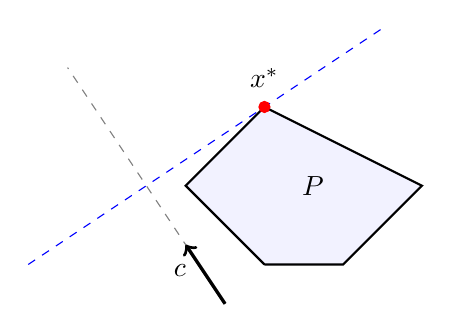
\begin{tikzpicture}[scale=1]
\draw[color=black, fill=blue!5, thick] (0,0)--(1,0)--(2,1)--(0,2)--(-1,1)--(0,0);
\draw[color=black!50,dashed] (-0.5,-0.5)--(-2.5,2.5);
\draw[color=black,very thick,->] (-0.5,-0.5)--(-1,0.25);
\draw[color=blue,dashed] (-3,0)--(1.5,3);
\filldraw[red] (0,2) circle (2pt);
\node (A1) at (-0.75,0.25)  [label=225:{$\vct{c}$}] {};
\node (A2) at (1,1)  [label=180:{$P$}] {};
\node (A3) at (0,2)  [label=90:{$\vct{x}^*$}] {};
\end{tikzpicture}
\caption{Geometry of linear programming} \label{fig:geomlinprog}
\end{figure}

The famous duality theorem for linear programming states that if the maximum of~\eqref{eq:linprog} exists, then it coincides with the solution of a {\em dual} linear programming problem.

\begin{theorem}\label{thm:duality}
Let $\mtx{A}\in \R^{m\times n}$, $\vct{b}\in \R^m$ and $\vct{c}\in \R^n$. Then
the optimal value of
\begin{equation}\label{eq:primal}\tag{P}
 \maximize \ip{\vct{c}}{\vct{x}} \ \subjto \mtx{A}\vct{x}\leq \vct{b}
\end{equation}
coincides with the optimal value of
\begin{equation}\label{eq:dual}\tag{D}
 \minimize \ip{\vct{b}}{\vct{y}} \ \subjto \mtx{A}^{\trans}\vct{y}=\vct{c}, \  \vct{y}\geq \zerovct,
\end{equation}
provided both~\eqref{eq:primal} and ~\eqref{eq:dual} have a finite solution.
\end{theorem}

The problem~\eqref{eq:primal} is called the {\em primal} problem, and~\eqref{eq:dual} the {\em dual} problem.

\begin{example}
 Consider the simple problem
 \begin{equation*}
  \maximize x_1 \ \subjto x_1+x_2\leq 1, x_1\geq 0, x_2\geq 0.
 \end{equation*}
The dual problem is
\begin{equation*}
 \minimize y_1 \ \subjto y_1-y_2=1, y_1-y_3=0, y_1\geq 0, y_2\geq 0, y_3\geq 0. 
\end{equation*}
\end{example}

For the proof we need the following observation.

\begin{lemma}
 Let $P\subset \R^n$ be a polyhedron and $\vct{c}\in \R^n$ such that $\sup_{\vct{x}\in P}\ip{\vct{c}}{\vct{x}}$ is finite. Then the supremum is attained, that is, it is a maximum.
\end{lemma}

\begin{proof}[Proof of Theorem~\ref{thm:duality}]
 Let $P=\{\vct{x}\mid \mtx{A}\vct{x}\in \vct{b}\}$ and $D=\{\vct{y}\in \R^m\mid \mtx{A}^{\trans}\vct{y}=\vct{c}, \vct{y}\geq \zerovct\}$. If $\vct{x}\in P$ and $\vct{y}\in Q$, then
 \begin{equation*}
  \ip{\vct{c}}{\vct{x}} = \ip{\mtx{A}^{\trans}\vct{y}}{\vct{x}} = \ip{\vct{y}}{\mtx{A}\vct{x}}\leq \ip{\vct{y}}{\vct{b}},
 \end{equation*}
so that in particular
\begin{equation*}
 \max_{\vct{x}\in P}\ip{\vct{c}}{\vct{x}}\leq \min_{\vct{y}\in Q}\ip{\vct{b}}{\vct{y}},
\end{equation*}
which shows one inequality. To show the other inequality, set $\delta = \max_{\vct{x}\in P} \ip{\vct{c}}{\vct{x}}$. By definition, if $\mtx{A}\vct{x}\leq \vct{b}$, then $\ip{\vct{c}}{\vct{x}}\leq \delta$. By Corollary~\ref{cor:farkas3}, there exists a vector $\vct{y}\in \R^m$ such that
\begin{equation*}
 \vct{y}\geq \zerovct, \quad \mtx{A}^{\trans}\vct{y}=\vct{c}, \quad \ip{\vct{b}}{\vct{y}}\leq \delta.
\end{equation*}
In particular,
\begin{equation*}
 \min_{\vct{y}\in Q} \ip{\vct{b}}{\vct{y}}\leq \delta = \max_{\vct{x}\in P}\ip{\vct{c}}{\vct{x}}.
\end{equation*}
This finishes the proof.

\end{proof}


% %-----------------------------------------------------------------------
% % End of chap1.tex
% %-----------------------------------------------------------------------
